\chapter{国内外研究现状}

本章介绍与本文相关的三个主题:深度学习、度量学习、对抗样本问题。本文研究的是如何结合度量学习的思想以缓和深度学习中的对抗样本问题,我们针对的主要是比较基础的图像分类任务,其它任务中的对抗样本问题不在本文讨论范畴,但值得进一步推广和探索。

\section{深度学习}

2006年,多伦多大学教授Geoffrey Hinton及其学生Rusian发表在世界顶级学术期刊《科学》上的一篇论文引发了深度学习在研究领域和应用领域的发展热潮\cite{hinton2006reducing}。这篇文献提出了两个主要观点:(1)、多层人工神经网络有很强的特征学习能力,深度学习模型学习得到的特征数据对原数据有更本质的代表性,这将大大便于分类和可视化问题;(2)、对于深度神经网络难以训练的问题,可以采用逐层训练的方法解决。

深度学习发展到今天,已经在许多领域大放异彩,例如:计算机视觉、自然语言处理、医学影像分析、语音、游戏、图网络、时间序列、机器人控制、计算机编程等。本节主要介绍深度学习在图像分类(Image classification)和目标检测(Object detection)上的进展。

\subsection{图像分类}

早在1989年,受到生物学家Hubel和Wiesel的动物视觉模型\cite{hubel1962receptive}的启发,Yann LeCun等人就提出了一个多层的卷积神经网络(Convolutional Neural Network, CNN)\cite{lecun1989backpropagation}。但由于优化方法、数据量和计算能力等限制,直到2012年,Hinton等人才采用更深的卷积神经网络模型AlexNet在著名的ImageNet问题上取得当时世界上最好的成果,使得对于图像识别的研究工作前进了一大步\cite{krizhevsky2012imagenet}。

\begin{figure}[h]
    \centering
    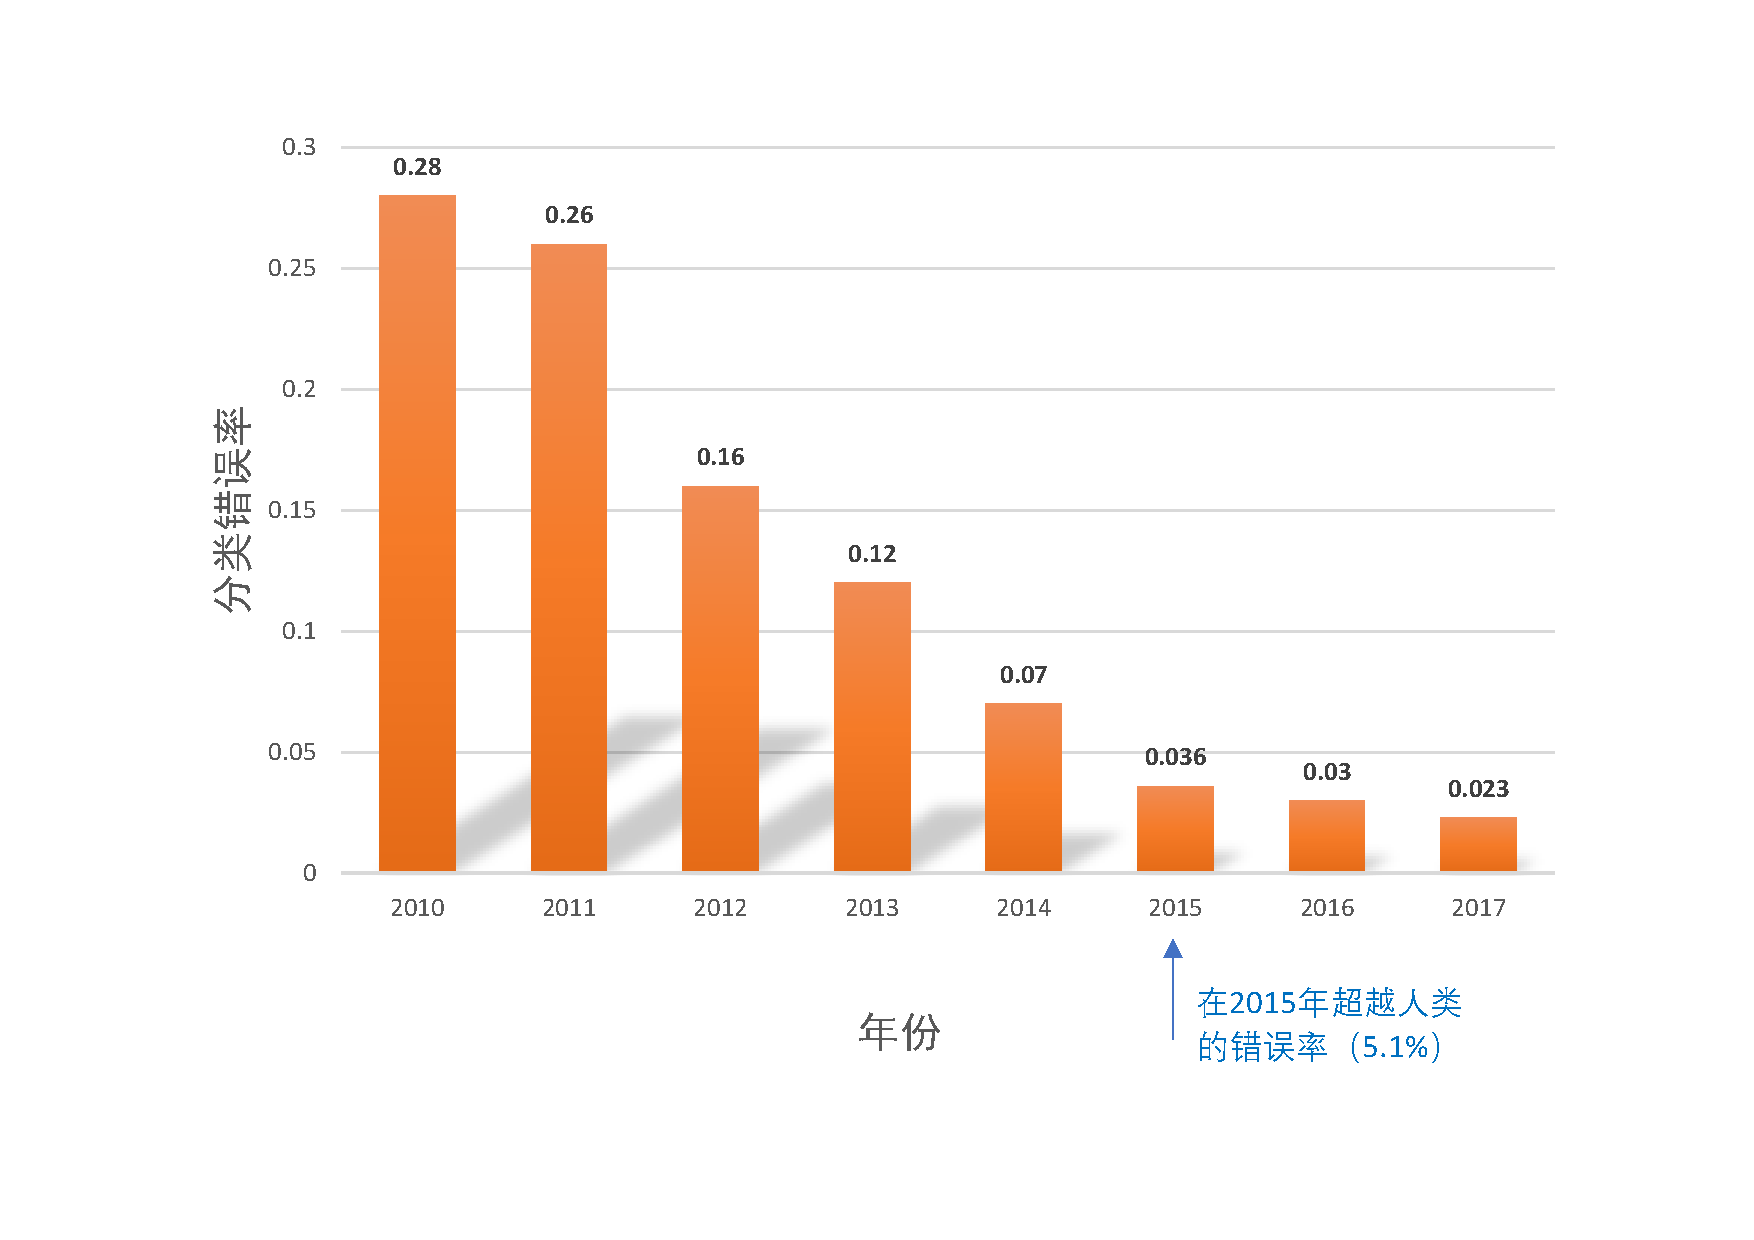
\includegraphics[width=15cm]{fig/imagenet.pdf}
    \caption{2010 $\sim$ 2017年ImageNet分类任务错误率}
    \label{fig:imagenet}
\end{figure}

2014年,更深的深度网络VGGNet\cite{simonyan2014very}和GoogLeNet\cite{szegedy2015going}被成功训练,分别为16层和22层。2015年,He等人提出ResNet\cite{he2016deep},利用残差单元(Residual unit)有效地缓和了梯度消失问题,成功训练了一个152层的深度神经网络,进一步提高了在ImageNet上的分类性能。2017年,注意力机制被引入深度网络架构中,Hu等人提出SENet\cite{hu2018squeeze},利用通道间的自注意力机制,赢得了最后一届ImageNet竞赛的冠军。随后Woo等人提出CBAM模块\cite{woo2018cbam},结合通道间和空间的自注意力,进一步提升了性能。\autoref{fig:imagenet}展示了2010 $\sim$ 2017年ImageNet分类错误率变化情况,从错误率的指标上看,深度网络已经超越人类。

\subsection{目标检测}

自从AlexNet获得ILSVRC 2012挑战赛冠军后,用CNN进行分类成为主流。2014年,Girshick等人提出R-CNN\cite{girshick2014rich},利用候选区域方法(Region proposal method)创建目标检测感兴趣的区域(Resion of Interest, ROI),再送入CNN进行分类,此方法每预测一张图片需要49秒。2015年,Ross Girshick提出Fast R-CNN\cite{girshick2015fast},利用特征图代替原图生成ROI,显著地减少处理时间至每张图片2.3秒。2016年,Ren等人提出Faster R-CNN\cite{ren2015faster},使用内部的候选区域网络代替了外部的候选区域方法,使得ROI的生成效率进一步提高,每张图片的处理时间减小到0.2秒。

以上的目标检测器由于候选区提取和分类是分开做的,被称为二次检测器(Two-stage detector),与之对应的是随后提出的单次检测器(One-stage detector)。Liu等人提出的SSD模型\cite{liu2016ssd}和Redmon等人提出的YOLO模型\cite{redmon2016you, redmon2017yolo9000, redmon2018yolov3}将候选区提取和分类用端到端(End-to-end)的方式融合到一起训练,使得目标检测器真正达到了实时检测的程度,但对小目标的检测效果较差。Lin等人提出特征金字塔网络(Feature Pyramid Network, FPN)\cite{lin2017feature},利用多尺度特征图提高准确率。

\section{度量学习}

过去的十几年里,大量的度量学习(Metric Learning)算法被提出,其中最典型的是对比损失(Contrastive loss)\cite{chopra2005learning, hadsell2006dimensionality}和三元组损失(Triplet loss)\cite{weinberger2009distance, chechik2010large}。它们的目标通常是学习一个良好的距离度量,使得正样本对(Positive pair)之间的距离尽量小,负样本对(Negative pair)之间的距离尽量大。这些度量学习方法被提出时,只能够学习一个线性变换,无法很好地刻画现实数据中的非线性流形结构。为了解决这个问题,核技巧通常被采用,先将样本映射到一个高维的特征空间中,然后再在这个高维空间里学习一个距离度量\cite{tsang2003distance, yeung2007kernel}。然而,这些方法无法显式地得到一个非线性映射函数,因此无法被应用到更大规模的数据上。

自深度学习表现出强大的表示学习能力之后,深度神经网络便被引入到度量学习之中,以学习一个非线性映射。Hu等人将深度网络应用到对比损失中\cite{hu2014discriminative},Hoffer等人将深度网络应用到三元组损失中\cite{hoffer2015deep}。然而,将深度网络直接地应用到度量学习中,带来的问题是:这些方法随机采样样本对或三元组以构成训练批次,无法在小批次随机梯度下降的训练过程中充分利用一批次里的所有训练样本。Kihyuk和Oh Song等人分别提出一种新颖的采样方式\cite{oh2016deep, sohn2016improved},能够充分利用小批次里的所有样本,提升了深度度量学习(Deep Metric Learning)的性能。

\section{对抗样本问题}

早在十几年前,对抗样本问题就在传统机器学习中被讨论过。2004年,Dalvi等人首次讨论了对抗样本,把这个问题看做敌人和分类器之间的一个博弈问题\cite{dalvi2004adversarial},在对抗样本上的攻击和防御变成了一场迭代式的博弈。通过增加字符以避免检测,对抗攻击曾被应用到垃圾邮件过滤系统中\cite{dalvi2004adversarial, biggio2010multiple}。2013年,Biggio等人首先提出一个基于梯度的方法生成对抗样本以攻击浅层的分类器,比如支持向量机、一个两层的神经网络\cite{biggio2013evasion}。与深度学习中的对抗样本相比,传统机器学习中的方法在修改数据上拥有更大的自由度,第一个被用来评估攻击方法的数据集是MNIST,但此时生成的对抗样本能被人类轻易地分辨出来。

在传统机器学习中,攻击和防御方法都在特征提取过程中下了很大功夫,甚至可以影响数据采集过程,在对人类的影响上并没有太多的考虑\cite{roli2013pattern};而在深度学习中,只需要关心原始数据的输入,且非常强调对人类视觉系统的影响。

本文重点研究图像分类任务中的对抗样本:使用一个第三方发布的预训练的分类器,用户输入一张图片以得到分类器的预测结果。对抗样本是在干净的原始样本上添加一些微小的扰动,这些扰动通常无法被人类感知到。然而,这样的扰动可以误导图片分类器,用户将得到一个不正确的预测结果。记$f$为一个训练好的深度学习模型,$x$为一个原始的输入样本数据,一个对抗样本$x'$的生成过程可以被描述为一个带约束的优化问题:
\begin{equation}
    \begin{aligned}
    \min_{x^{\prime}} \quad & \left\|x^{\prime}-x\right\| \\
    s.t. \quad & f\left(x^{\prime}\right)=l^{\prime}, \\ 
               & f(x)=l, \\ 
               & l \neq l^{\prime}, \\ 
               & x^{\prime} \in[0,1],
\end{aligned}
\end{equation}
其中$l$和$l'$表示$x$和$x'$的输出标记,$\|\cdot\|$表示两个样本点之间的距离,$\eta=x'-x$表示添加在$x$上的扰动。这个优化问题在输入数据有范围限制的情况下,误导模型预测结果的同时最小化扰动。

\subsection{攻击方法}

2014年,Szegedy等人首先提出了针对深度神经网络的对抗样本,提出了一种名为L-BFGS的攻击方法。L-BFGS方法使用代价较高的线性搜索方法去寻找参数的最优值,这非常耗时且实用性不强,因此Goodfellow等人提出了一个快速的生成对抗样本的方法,称作快速梯度符号方法(Fast Gradient Sign Method, FGSM),此方法仅仅只需要沿着每个像素的梯度符号方向执行一步梯度更新,便可生成如\autoref{fig:adversarial_example}所示的对抗样本\cite{goodfellow2014explaining}。2016年,Kurakin等人为了将对抗样本应用到物理世界中,他们扩展了FGSM方法,使用更细化的优化过程和多次的迭代以生成更具有迁移能力的对抗样本,称作基本迭代方法(Basic Iterative Method, BIM),成功欺骗了一个运行在手机上的ImageNet分类器\cite{kurakin2016adversarial}。Moosavi-Dezfooli等人提出DeepFool方法以寻找与原始样本距离最小的对抗样本\cite{moosavi2016deepfool}。2017年,Carlini和Wagner提出了一个非常强大的攻击方法C\&W's Attack,使得许多防御方法失效\cite{carlini2017towards}。Chen等人提出一种基于零阶优化(Zeroth Order Optimization, ZOO)的攻击方法,这个方法不需要梯度信息,所以可以被直接应用到黑盒攻击上,无需迁移\cite{chen2017zoo}。Moosavi-Dezfooli等人基于DeepFool提出了一种普适性的对抗攻击(Universal adversarial attack),能够找到攻击尽量多样本的一个普适性的扰动。为了让人类无法察觉对抗扰动,Su等人提出单像素攻击(One pixel attack),利用进化算法寻找一个像素点进行扰动\cite{su2019one}。

在视觉应用方面。2016年,Sharif等人设计了一个眼镜形状的对抗扰动,以攻击基于深度神经网络的人脸识别系统\cite{sharif2016accessorize}。2017年,Xie等人提出密集敌人生成(Dense Adversary Generation, DAG)算法,能够生成针对目标检测和语义分割系统的对抗样本\cite{xie2017adversarial}。2019年,腾讯科恩实验室对特斯拉Autopilot自动驾驶系统的安全性进行研究,成功攻击了Autopilot系统的外部天机状况识别系统和道路交通标线识别系统,分别使得车辆雨刷误启动和驶入反向车道\cite{tecent2019tesla}。

在自然语言处理应用方面。2017年,针对阅读理解系统,为了产生与正确答案一致且不混淆人的对抗性例子,Jia等人在段落末尾增加了对抗性字段\cite{jia2017adversarial}。2019年,针对语音识别系统,Qin等人提出了一种有效的人类不可察觉的音频对抗样本生成方法,此方法充分利用了听觉掩模的心理声学原理,对任意的全语句目标都达到了百分之百的攻击成功率,进一步,他们发现在物理世界中通过空气传播此对抗音频后,攻击仍然有效\cite{qin2019imperceptible}。

\subsection{防御方法}

2016年,Papernot等人提出使用网络蒸馏(Network distillation)作为一个防御对抗样本的手段\cite{papernot2016distillation},但随后被Carlini等人提出的C\&W's Attack成功击破。2017年,许多检测方法被用来检测对抗样本。有的工作提出使用一个基于深度网络的二元分类器用于检测并过滤对抗样本\cite{lu2017safetynet, metzen2017detecting, gong2017adversarial},有的工作提出添加一个离群类到原始的深度学习模型中以检测并过滤对抗样本\cite{grosse2017statistical},还有的工作发现对抗样本的分布与干净样本的不同,提出用基于PixelCNN\cite{Salimans2017pixelcnn}排序的p值进行对抗样本的检测和拒绝\cite{song2017pixeldefend}。然而,Carlini和Wagner总结了以上对抗性的检测方法,展示了这些检测防御方法都可以被更具有针对性的攻击轻易规避\cite{carlini2017adversarial, carlini2017magnet}。2018年,许多梯度掩码(Gradient masking)的方法被提出用来增强深度网络的鲁棒性。Jacob等人提出用温度计编码(Thermometer encoding)来提高鲁棒性\cite{buckman2018thermometer};Guo等人提出将输入的图片进行五个预变换,以消除对抗扰动,提升模型鲁棒性\cite{guo2018countering};Dhillon等人提出随机激活剪枝(Stochastic Activation Pruning, SAP),随机抛弃部分神经元以消除对抗扰动的影响\cite{s.2018stochastic};Xie等人提出在输入样本被送入模型前对样本进行随机变换,以消除对抗扰动的影响\cite{xie2018mitigating};Song等人提出使用PixelCNN模型将潜在的对抗样本投影到真实的数据流形上以消除对抗扰动\cite{song2018pixeldefend};Samangouei等人提出使用生成对抗网络将样本投影到生成器的数据流形中以消除对抗扰动\cite{samangouei2018defensegan};然而,以上所有梯度掩码的方法都被Athalye等人使用具有针对性的攻击方法一一破解\cite{pmlr-v80-athalye18a}。

同时,Athalye等人也指出,目前只有对抗训练这一种防御方式无法被完全击破,但对抗训练也有自身的问题\cite{pmlr-v80-athalye18a}。虽然对抗训练在MNIST上的鲁棒性比较令人满意\cite{madry2018towards},但在ImageNet这样的数据集上的鲁棒性就差强人意了\cite{kurakin2017adversarial}。而且对抗训练在CIFAR10和ImageNet上的泛化性能比较差,这个泛化性能包括在测试时对同一种攻击方式(与训练时使用的攻击方式相同)的鲁棒性和测试时对其它攻击方式(与训练时使用的攻击方式不同)的鲁棒性,通常认为对抗训练的样本复杂度远高于自然训练的样本复杂度\cite{schmidt2018adversarially}。

为了提高对抗训练的泛化能力,Kannan等人提出对抗逻辑配对(Adversarial Logit Pairing),提高了对抗训练在ImageNet上的泛化能力\cite{kannan2018adversarial},并被NIPS 2018接收,但随后被人指出并实验上证明了该方法并没有真正地提在ImageNet上的泛化能力\cite{engstrom2018evaluating},于是ALP又被作者从NIPS上撤稿。本文也对ALP的有效性进行了一些探究,详见章节\ref{section:generalization}。Song等人提出使用将干净样本分类和对抗样本分类看做一个域适应的问题,采用最大均值散度(Maximum Mean Discrepancy, MMD)和相关性匹配(CORrelation ALignment, CORAL)作为正则化项提高对抗训练的泛化能力\cite{song2018improving}。Farnia等人提出使用谱归一化来提高对抗训练的泛化能力\cite{farnia2018generalizable}。